% \documentclass[aspectratio=169, 11pt]{beamer}
\documentclass[aspectratio=169, 11pt, handout]{beamer}

% Version 2 (2026-09-28). Restructured on the course spine: estimand -> identification -> estimation
% (course-spine.md). Changes from slides.tex are listed in m02/CHANGES-v2.md.

% ── Theme ──
\usetheme{Madrid}
\usecolortheme{default}
\setbeamertemplate{navigation symbols}{}
\setbeamertemplate{footline}{%
  \leavevmode\hbox{%
    \begin{beamercolorbox}[wd=.333333\paperwidth,ht=2.5ex,dp=1ex,center]{author in head/foot}%
      \usebeamerfont{author in head/foot}\insertshortauthor
    \end{beamercolorbox}%
    \begin{beamercolorbox}[wd=.333333\paperwidth,ht=2.5ex,dp=1ex,center]{title in head/foot}%
      \usebeamerfont{title in head/foot}\insertshorttitle
    \end{beamercolorbox}%
    \begin{beamercolorbox}[wd=.333333\paperwidth,ht=2.5ex,dp=1ex,right]{date in head/foot}%
      \usebeamerfont{date in head/foot}\insertframenumber{} / \inserttotalframenumber\hspace*{2ex}
    \end{beamercolorbox}}}

% ── Packages ──
\usepackage{amsmath,amssymb}
\usepackage{booktabs}
\usepackage{xcolor}
\usepackage{colortbl}
\usepackage{graphicx}
\usepackage{tikz}
\usetikzlibrary{arrows.meta, positioning, calc}

% ── Colors ──
\definecolor{sbgreen}{HTML}{00704A}  % course accent
\definecolor{warnred}{HTML}{CC0000}
\definecolor{noteblue}{HTML}{2060A0}

% ── Commands ──
\newcommand{\E}{\mathbb{E}}
\newcommand{\Var}{\mathrm{Var}}
\newcommand{\Cov}{\mathrm{Cov}}
\newcommand{\SE}{\mathrm{SE}}
\newcommand{\Prob}{\mathrm{Pr}}
\newcommand{\indep}{\perp\!\!\!\perp}
\usepackage{soul}
\newcommand{\NUM}[2]{\sethlcolor{yellow}\hl{#1\,\textsuperscript{?}}\marginpar{\tiny #2}}
% Beamer frames are typeset inside boxes, where \marginpar raises "Not in outer par mode"
% and \marginparwidth is 4pt. Same marker; the provenance note goes to the frame footnote.
\renewcommand{\NUM}[2]{\sethlcolor{yellow}\hl{#1\,\textsuperscript{?}}\footnote[frame]{\tiny #2}}
% Compact footnote layout so several provenance notes fit under one frame.
\setbeamertemplate{footnote}{\noindent\raggedright\hspace*{0.6em}\tiny\insertfootnotemark\,\insertfootnotetext\par}

% Step labels for the course spine
\newcommand{\spinestep}[1]{\textcolor{sbgreen}{\textbf{#1}}}

% ── Title ──
\title[Meeting 2]{Meeting 2: Real, Profitable, and Where It Holds}
\subtitle{Applied Causal Inference for Business}
\author{Zhikun Lu}
\date{\today}

\begin{document}

% ====================================================================
\begin{frame}
\titlepage
\end{frame}

% ====================================================================
\begin{frame}{Where Does the Counterfactual Come From?}

\begin{center}
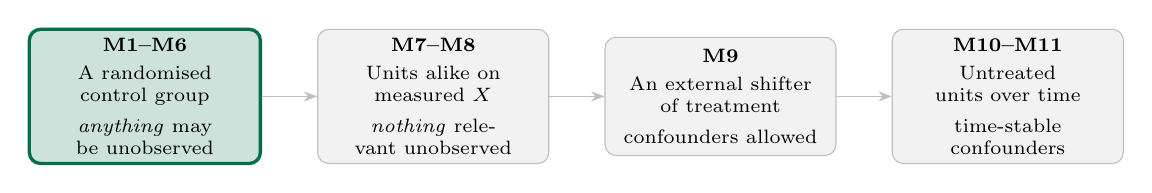
\begin{tikzpicture}[
    node distance=0.45cm and 0.7cm,
    box/.style={draw, rounded corners, minimum width=2.9cm, minimum height=1.5cm,
                font=\scriptsize, align=center, text width=2.7cm},
    active/.style={box, fill=sbgreen!20, draw=sbgreen, very thick},
    inactive/.style={box, fill=gray!10, draw=gray!50}
]
\node[active] (A) {\textbf{M1--M6}\\[2pt] A randomised control group\\[3pt] \emph{anything} may be unobserved};
\node[inactive, right=of A] (B) {\textbf{M7--M8}\\[2pt] Units alike on measured $X$\\[3pt] \emph{nothing} relevant unobserved};
\node[inactive, right=of B] (C) {\textbf{M9}\\[2pt] An external shifter of treatment\\[3pt] confounders allowed};
\node[inactive, right=of C] (D) {\textbf{M10--M11}\\[2pt] Untreated units over time\\[3pt] time-stable confounders};
\draw[-{Stealth}, gray!50] (A) -- (B);
\draw[-{Stealth}, gray!50] (B) -- (C);
\draw[-{Stealth}, gray!50] (C) -- (D);
\end{tikzpicture}
\end{center}

\bigskip

\begin{center}
\small Last time the coin removed the bias. It did not remove the \emph{luck}: one draw, one estimate.\\
Today: how far one draw can mislead, where its answer applies, and how to design the next one.
\end{center}
\end{frame}

% ====================================================================
\begin{frame}{Today's Plan}

\begin{center}
\small
\begin{tabular}{rp{11.6cm}}
\toprule
\textbf{Minutes} & \\
\midrule
0--15 & \textbf{Reading and critique C1} --- on paper, no devices \\
15--50 & The Q2 test, read two ways. \spinestep{Estimand} and \spinestep{estimation}: uncertainty from the draw --- Fisher, then Neyman \\
60--110 & Significant is not profitable; a second campaign (\spinestep{a new estimand}: transport); designing the next test --- power, CUPED, the unit of assignment \\
120--180 & \textbf{Lab 1:} prompt specifications; generated estimators tested against a known effect and against your M1 estimator \\
\bottomrule
\end{tabular}
\end{center}

\bigskip

\textbf{Case:} Lin's coupon programme, Meeting 2 (Releases 1--4). \quad \textbf{Today:} form project pairs; P1 released.

\bigskip

\textbf{Reading:} technical notes for Meeting 2. Section 1 is examinable.
\end{frame}

% ====================================================================
\begin{frame}{Critique C1: Five Questions, Every Time}

Read the one-page case silently. Notes on your own, then pairs, then the room.

\bigskip

\begin{enumerate}
    \item What is the claim?
    \item What causal question does the decision need?
    \item Who is the comparison group?
    \item What else could produce this pattern? Give the mechanism and the \textbf{direction} of the bias.
    \item What would you do to find out?
\end{enumerate}

\bigskip

\small Questions 2 and 3 are Meeting 1's steps 1 and 2: the estimand, and where the counterfactual comes from. Hand in your notes at minute 15.
\end{frame}

% ====================================================================
\section{The Test Is Back}
% ====================================================================

% [RELEASE R1 — the Q2 result and the two readings of it]
\begin{frame}{The Q2 Test, Read Two Ways}

In the 1{,}000-member test region, 500 members were drawn at random for the \textyen 10 coupon.

\begin{center}
\begin{tabular}{lrrr}
\toprule
& \textbf{Members} & \textbf{Bought} & \textbf{Purchase rate} \\
\midrule
Coupon & 500 & 250 & 0.50 \\
No coupon & 500 & 200 & 0.40 \\
\bottomrule
\end{tabular}
\end{center}

\bigskip

\textbf{Marketing:} \emph{``It was randomised, and it's significant. The coupon works. Roll it out.''}

\medskip

\textbf{The CFO:} \emph{``Last week you said it loses \textyen 2 a coupon. Which is it?''}

\bigskip

Both can be true. They answer different questions, and each answer comes from \textbf{one draw of the coin}. Before anyone rolls anything out, we need to know how far one draw can mislead.
\end{frame}

% ====================================================================
\begin{frame}{The Number That Decides It}

From M1: with \textyen 30 margin and a \textyen 10 coupon paid on every holder's purchase,

\begin{alertblock}{Break-even lift}
\[
\tau^{*} = \frac{p_1}{3} = \frac{0.50}{3} = \mathbf{0.167}
\]
\end{alertblock}

\bigskip

Two different null hypotheses, two different decisions:

\begin{center}
\begin{tabular}{lll}
\toprule
\textbf{Question} & \textbf{Null} & \textbf{Who asks} \\
\midrule
Does the coupon do anything? & $\tau = 0$ & marketing \\
Does the coupon pay? & $\tau \leq 0.167$ & the CFO \\
\bottomrule
\end{tabular}
\end{center}

\bigskip

Every estimate today comes with an interval. The only question is \textbf{where the interval sits relative to $0$ and to $0.167$}.
\end{frame}

% ====================================================================
\begin{frame}{What Exactly Are We Uncertain About?}

\spinestep{Estimand.} $\tau_S = \frac{1}{1000}\sum_i \{Y_i(1) - Y_i(0)\}$ for the 1{,}000 members of the region: \textbf{a fixed number}. \\
\spinestep{Identification} (M1): the draw makes $\bar Y_1 - \bar Y_0$ unbiased for it.

\bigskip

So where does uncertainty come from? Two answers:

\medskip

\begin{center}
\begin{tabular}{p{3.2cm}p{4.6cm}p{4.6cm}}
\toprule
& \textbf{Design-based} (today first) & \textbf{Superpopulation} \\
\midrule
Customers & fixed: these 1{,}000 & a random sample from a larger population \\
Random & only the coin & the coin \emph{and} the sample \\
Estimand & $\tau_S$, this region & the population's ATE \\
Needs & nothing but the draw log & a sampling assumption \\
\bottomrule
\end{tabular}
\end{center}

\bigskip

\small Your M1 workshop drew the design-based distribution directly: customers fixed, the coin redrawn 200 times.
\end{frame}

% ====================================================================
\section{Uncertainty From the Draw}
% ====================================================================

% [CONDENSED from old-decks/lecture01.tex (tea) and lecture02 urn frames]
\begin{frame}{Fisher: Is the Difference Real or Just the Draw?}

\textbf{Sharp null:} the coupon does nothing for \emph{anyone}, $Y_i(1) = Y_i(0)$ for every $i$.

\medskip

Then every member's outcome is known under both labels: 450 buyers, 550 non-buyers, whatever the coin said. \textbf{The only random element is which 500 the draw labelled ``coupon''.}

\bigskip

\begin{columns}[T]
\begin{column}{0.46\textwidth}
\small
\textbf{Tea (Fisher, 1935).} 8 cups, 4 milk-first. Under ``she is guessing'', all $\binom{8}{4} = 70$ labellings are equally likely; a perfect score has probability $1/70 = 0.014$.
\end{column}
\begin{column}{0.50\textwidth}
\small
\textbf{Coupon.} Under the sharp null, $\bar Y_1 - \bar Y_0$ over all possible draws has mean 0 and, with the pooled rate $\hat p = 0.45$,
\[
\SE_0 = \sqrt{\tfrac{2(0.45)(0.55)}{500}} = 0.0315 ,
\]
so $z = 0.10/0.0315 = 3.17$, $p \approx 0.0015$.
\end{column}
\end{columns}

\bigskip

\textbf{Reject: the coupon does something for someone.} No model, no sampling assumption --- only the draw. But it answers only ``is it zero for \emph{everyone}?'', and its SE is computed assuming that answer. For an interval around an average effect, we need Neyman.
\end{frame}

% ====================================================================
\begin{frame}[shrink=10]{Neyman: How Far Does One Draw Land?}

Customers fixed, only the coin random. Over all possible draws, exactly:
\[
\Var_D(\widehat\tau) = \frac{S_1^2}{n_1} + \frac{S_0^2}{n_0} - \frac{S_\tau^2}{n} ,
\]
with $S_1^2, S_0^2$ the spreads of $Y(1)$ and $Y(0)$ across the 1{,}000 members, and $S_\tau^2$ the spread of their individual effects.

\bigskip

\textbf{The last term needs both potential outcomes of each member --- never observed.} Drop it:
\[
\widehat\SE = \sqrt{\frac{\hat p_1(1-\hat p_1)}{n_1} + \frac{\hat p_0(1-\hat p_0)}{n_0}} = \sqrt{\frac{0.25}{500} + \frac{0.24}{500}} = \mathbf{0.0313}
\]

\begin{block}{The standard SE is conservative for a fixed population}
On M1's type table, $\sqrt{0.000500 + 0.000480 - 0.000290} = \mathbf{0.026}$: the spread of your 200 workshop draws. The usual formula says $0.031$. The gap is effect heterogeneity we cannot see.
\end{block}

\small If the customers were instead a random sample from a larger population, the same $\widehat\SE$ is the right one for that population's ATE.
\end{frame}

% [REVISED from old-decks/lecture01.tex:531]
\begin{frame}{Testing and the Confidence Interval}

$z$-statistic against zero, with the Neyman SE:
\[
z = \frac{\hat{\tau}}{\widehat{\SE}} = \frac{0.10}{0.0313} \approx 3.19, \qquad \text{p-value} \approx 0.0014
\]

\bigskip

95\% confidence interval:
\[
\hat{\tau} \pm 1.96 \times \widehat{\SE} = 0.10 \pm 0.061 = [0.039, \; 0.161]
\]

\bigskip

\textbf{What the 95\% means:} across repeated draws of the coin, about 95\% of intervals built this way would contain $\tau_S$ --- at least 95\%, since the SE is conservative. It is \emph{not} a 95\% probability that this interval contains a fixed number.

\bigskip

\begin{block}{Two statements, always both}
The test says whether the difference is \textbf{distinguishable from the draw}. The interval says \textbf{how big} the effect plausibly is. The interval is the set of nulls the test does not reject.
\end{block}
\end{frame}

% ====================================================================
\begin{frame}{Analyse as Drawn}

Marketing proposes a ``cleaner'' comparison: drop members who never opened the app during the test --- \emph{``they never saw the coupon''}.

\bigskip

\begin{itemize}
    \item Opening the app is measured \textbf{after} the draw, and the coupon notification makes it more likely: it is post-treatment (M1's data roles).
    \item Dropping non-openers keeps different people in the two arms. The coin no longer decides who is compared.
\end{itemize}

\bigskip

\begin{block}{Compare the arms as the coin made them}
The difference over \emph{all} drawn members is the effect of \textbf{sending} the coupon --- the intention-to-treat effect. It is also the decision: the chain controls sending, not reading.
\end{block}

\small The effect of \emph{receiving} it is a different estimand, with its own identification. M9.
\end{frame}

% ====================================================================
\section{Significant Is Not Profitable}
% ====================================================================

\begin{frame}{Test Against the Break-Even, Not Against Zero}

Same estimate, same $\widehat\SE = 0.0313$, a different null:
\[
H_0 : \tau \leq \tau^* = 0.167 \;\; \text{(does not pay)}, \qquad
z = \frac{0.10 - 0.167}{0.0313} = -2.13
\]

The estimate is \textbf{two standard errors below} break-even. And the 95\% interval $[0.039,\, 0.161]$ excludes \emph{both} $0$ and $0.167$.

\begin{center}
\small
\begin{tabular}{ll}
\toprule
\textbf{Where the interval sits} & \textbf{Decision} \\
\midrule
Entirely above $\tau^*$ & Roll out \\
Straddles $\tau^*$ & Undecided on profit: a bigger or sharper test \\
Between $0$ and $\tau^*$ & \textcolor{warnred}{It works and it does not pay} \quad $\leftarrow$ Q2 \\
Includes $0$ & Cannot yet tell it works \\
\bottomrule
\end{tabular}
\end{center}

Marketing and the CFO were both right. ``Significant'' answered marketing's question. It was never the decision.
\end{frame}

% ====================================================================
\begin{frame}{Test the Profit Directly}

The break-even used $\hat p_1 = 0.50$, which is \emph{itself} an estimate. Put the decision variable on the left --- M1's per-type margins, averaged:
\[
\text{net} = 30\tau - 10\,p_1 = 20\,p_1 - 30\,p_0
\qquad\Longrightarrow\qquad
\widehat{\text{net}} = 20(0.50) - 30(0.40) = -\text{\textyen}2.00
\]

The same (conservative) variance calculation, with the coefficients squared:
\[
\Var(\widehat{\text{net}}) = 20^2 \times 0.0005 + 30^2 \times 0.00048 = 0.200 + 0.432 = 0.632,
\qquad \widehat\SE = 0.795
\]

\begin{alertblock}{The number for the CFO}
\[
\text{net per coupon} = -\text{\textyen}2.00, \qquad 95\% \text{ CI } [-\text{\textyen}3.56,\; -\text{\textyen}0.44]
\]
\end{alertblock}

The whole interval loses money. \textbf{Put the uncertainty on the quantity the decision is made on} --- not only on the lift.
\end{frame}

% ====================================================================
\section{A Second Campaign: A New Estimand}
% ====================================================================

% [RELEASE R2 — two proposed second campaigns, each with its own randomised test]
\begin{frame}{Campaign A: The Active-Heavy List}

Regional managers propose a Q3 campaign on 600 members they call ``loyal'': 400 active, 200 lapsed. It will be tested properly --- a 50/50 draw \emph{within} the list. Segment effects from M1.

\begin{center}
\begin{tabular}{lcccc}
\toprule
& \textbf{On the list} & \textbf{Coupon} & \textbf{Control} & \textbf{Whole base} \\
\midrule
Active & 400 (67\%) & 200 & 200 & 5{,}000 (50\%) \\
Lapsed & 200 (33\%) & 100 & 100 & 5{,}000 (50\%) \\
\bottomrule
\end{tabular}
\end{center}

The draw is valid within the list, so the difference in means correctly estimates the list's effect:
\[
\tau_{\text{A}} = \tfrac{2}{3} \times 0.05 + \tfrac{1}{3} \times 0.20 = 0.10
\]

The whole base has $\tau = 0.50 \times 0.05 + 0.50 \times 0.20 = 0.125$.

\bigskip

$\tau_{\text{A}} < \tau$ because the list over-represents active customers. \textbf{Identification is fine; the estimand is this list's.}
\end{frame}

% ====================================================================
\begin{frame}{Campaign B: The Lapsed-Heavy List}

A second region proposes 600 members flagged ``lapsing'': 200 active, 400 lapsed. Also a proper 50/50 draw within the list.

\begin{center}
\begin{tabular}{lcccc}
\toprule
& \textbf{On the list} & \textbf{Coupon} & \textbf{Control} & \textbf{Whole base} \\
\midrule
Active & 200 (33\%) & 100 & 100 & 5{,}000 (50\%) \\
Lapsed & 400 (67\%) & 200 & 200 & 5{,}000 (50\%) \\
\bottomrule
\end{tabular}
\end{center}

\[
\tau_{\text{B}} = \tfrac{1}{3} \times 0.05 + \tfrac{2}{3} \times 0.20 = 0.15
\]

Now $\tau_{\text{B}} > \tau = 0.125$: the list over-represents lapsed customers, who respond more.

\begin{alertblock}{Lesson}
Both tests are internally valid. Each measures \emph{its list's} estimand. Carrying a number from one population to another is a \textbf{new estimand plus an assumption}.
\end{alertblock}
\end{frame}

% ====================================================================
\begin{frame}[shrink=3]{Transport the Effect --- and the Break-Even}

\spinestep{Assumption:} the coupon works the same within each segment wherever it is sent. Then any list's effect is its segment mix times the segment effects:
\[
\tau_{\text{list}} = \sum_s w_s\,\tau_s, \qquad p_{1,\text{list}} = \sum_s w_s\, \E[Y(1) \mid s], \qquad \tau^*_{\text{list}} = p_{1,\text{list}}/3
\]

\begin{center}
\small
\begin{tabular}{lrrrrr}
\toprule
\textbf{List} & \textbf{Active share} & $\tau$ & $p_1$ & $\tau^*$ & \textbf{Net per coupon} \\
\midrule
Active only & 1 & 0.050 & 0.800 & 0.267 & \textcolor{warnred}{$-$\textyen 6.50} \\
Campaign A & 2/3 & 0.100 & 0.633 & 0.211 & \textcolor{warnred}{$-$\textyen 3.33} \\
Whole base & 1/2 & 0.125 & 0.550 & 0.183 & \textcolor{warnred}{$-$\textyen 1.75} \\
Campaign B & 1/3 & 0.150 & 0.467 & 0.156 & \textcolor{warnred}{$-$\textyen 0.17} \\
Lapsed only & 0 & 0.200 & 0.300 & 0.100 & \textcolor{sbgreen}{$+$\textyen 3.00} \\
\bottomrule
\end{tabular}
\end{center}

Campaign B has a higher lift than the base and \textbf{still loses}: its break-even moved too. Transport the decision, not just the effect.

\medskip

\small The case says the Q3 campaign uses \emph{``the same coupon, in the same app, in the same quarter''}. That sentence is what licenses $\tau_s$ carrying over. It is also why the Q2 region's $-$\textyen 20{,}000 is only a forecast for the base.
\end{frame}

% ====================================================================
\section{Designing the Next Test}
% ====================================================================

% [RELEASE R3 — Lin's two proposed Q3 tests and the lapsed-member constraint]
\begin{frame}{The Next Test}

The Q2 test settled one question (do not coupon everyone). Lin proposes two Q3 tests for the questions it left open:

\begin{enumerate}
    \item \textbf{A lapsed-only coupon test.} Does the coupon pay on lapsed members? Planning value $\tau = 0.20$; break-even $0.10$.
    \item \textbf{An in-store BOGO promotion.} It runs on the menu board, so it cannot be sent to individuals.
\end{enumerate}

\bigskip

\textbf{The constraint:} the test window reaches about 350 lapsed members --- \textbf{175 per arm}.

\bigskip

\begin{alertblock}{The number that decides the design}
The test must be able to tell $0.20$ from $0.10$: its \textbf{minimum detectable effect} must be at most the gap to break-even, $0.10$.
\end{alertblock}
\end{frame}

% ====================================================================
\begin{frame}{Fix It in Writing Before the First Coupon Goes Out}

A randomised test can still be ruined by what happens around the draw.

\begin{center}
\small
\begin{tabular}{p{3.4cm}p{8.8cm}}
\toprule
\textbf{Fix in advance} & \textbf{For the lapsed test} \\
\midrule
Unit and allocation & member; 175 / 175 by seeded draw \\
Outcome and window & any purchase within 7 days, every drawn member \\
Decision threshold & test against $0.10$, not $0$; report net value \\
Sample size, stopping rule & 175 per arm; analyse once, at the end --- no peeking \\
Exposure logging, guardrails & coupon delivery logged; unsubscribe rate watched \\
\bottomrule
\end{tabular}
\end{center}

\bigskip

\textbf{Day-one check: sample-ratio mismatch.} If the arms are not close to 175 / 175, the draw or the logging is broken --- stop before reading any outcome.

\medskip

\small Industry experimentation teams publish checklists of this kind (Microsoft's ExP ``pre-experiment'' patterns). Project P4's planted problems come from this list.
\end{frame}

% ====================================================================
\begin{frame}{Power and the Minimum Detectable Effect}

For a two-sided test at level $\alpha$ with power $1 - \beta$, per arm:
\[
n = \frac{(z_{\alpha/2} + z_\beta)^2 \cdot (\sigma_1^2 + \sigma_0^2)}{\text{MDE}^2}
\qquad\Longleftrightarrow\qquad
\text{MDE} = (z_{\alpha/2} + z_\beta)\sqrt{\frac{\sigma_1^2 + \sigma_0^2}{n}}
\]

With $\alpha = 0.05$ and 80\% power, $z_{\alpha/2} + z_\beta = 1.96 + 0.84 = 2.80$: the MDE is \textbf{2.8 standard errors}.

\bigskip

\textbf{Check on Q2.} To detect $0.10$ with $\sigma_1^2 + \sigma_0^2 = 0.25 + 0.24 = 0.49$:
\[
n = \frac{2.80^2 \times 0.49}{0.01} = 384.2 \;\Rightarrow\; \mathbf{385} \text{ per arm (round up)}.
\]
Q2 had 500, so its MDE was $2.80 \times 0.0313 = 0.088$.

\bigskip

Q2 was built to tell $0.10$ from zero. For the CFO's question the gap is $0.167 - 0.10 = 0.067$, below its MDE: under 80\% power. It separated them on this draw anyway. Power is a property of the design \textbf{and of the question}.
\end{frame}

% ====================================================================
\begin{frame}{The Lapsed Test Is Too Small}

Planning values for lapsed members: $p_1 = 0.30$, $p_0 = 0.10$.
\[
\sigma_1^2 + \sigma_0^2 = 0.30(0.70) + 0.10(0.90) = 0.21 + 0.09 = 0.30
\]

\textbf{Needed} for an MDE of $0.10$:
\[
n = \frac{7.84 \times 0.30}{0.01} = 235.2 \;\Rightarrow\; \textcolor{warnred}{\mathbf{236} \text{ per arm}} \quad > \quad 175 \text{ available}
\]

\textbf{Available:} at 175 per arm,
\[
\text{MDE} = 2.80\sqrt{0.30/175} = 2.80 \times 0.0414 = \textcolor{warnred}{0.116} \quad > \quad 0.10 .
\]

\bigskip

Two ways out: wait a quarter for more lapsed members, or \textbf{make each member's observation carry more information}. The second costs nothing.
\end{frame}

% ====================================================================
\begin{frame}{CUPED on One Slide}

Let $X$ be a \textbf{pre-period} metric --- Q1 purchases --- fixed before the draw. Analyse
\[
Y^{\text{cv}} = Y - \theta\,(X - \bar X) \quad \text{instead of } Y .
\]

\textbf{Still unbiased.} $X$ was set before the draw, so the arms have the same $X$ \emph{on average over draws}; the correction has mean zero.

\textbf{Less variable.} $\Var(Y - \theta X)$ is minimised at $\theta^* = \Cov(Y, X)/\Var(X)$, giving $\Var(Y)\,(1 - \rho^2)$.

\bigskip

\textbf{It can move the estimate, too.} $\widehat\tau^{\text{cv}} = \widehat\tau - \theta(\bar X_1 - \bar X_0)$. In any one draw the arms differ a little in $X$; CUPED removes that chance imbalance. A shift in the point estimate is the method working, not failing.

\begin{alertblock}{Precision, not identification}
Identification came from the draw. CUPED is step 3 only --- and only if $X$ is pre-treatment. A post-treatment $X$ (M1's data roles; M7's controls) subtracts part of the effect.
\end{alertblock}
\end{frame}

% ====================================================================
\begin{frame}{CUPED on the Lapsed Test}

Among lapsed members in the Q2 data, Q1 purchases and the outcome correlate at \NUM{0.6}{sim coupon-q2 v1: corr(Q1 purchases, Q2 purchase) among lapsed members}.

\bigskip

At $\rho = 0.6$, every variance is multiplied by $1 - 0.36 = 0.64$:

\begin{center}
\begin{tabular}{lrr}
\toprule
& \textbf{Without CUPED} & \textbf{With CUPED} \\
\midrule
Needed per arm for MDE $0.10$ & 236 & $0.64 \times 235.2 = 151$ \\
MDE at 175 per arm & 0.116 & $2.80\sqrt{0.64 \times 0.30/175} = 0.093$ \\
\bottomrule
\end{tabular}
\end{center}

\bigskip

\textcolor{sbgreen}{\textbf{The test fits in the window.}} Same members, same coupon, same draw; the pre-period column did the work of 85 extra customers per arm.

\bigskip

The same regression you ran in M1, with one more column: $Y = \alpha + \tau D + \beta X + \varepsilon$. The coefficient on $D$ is the CUPED estimate up to how $\theta$ is fitted.
\end{frame}

% ====================================================================
\section{The Unit of Assignment}
% ====================================================================

% [RELEASE R4 — the in-store BOGO proposal]
\begin{frame}{Whose Outcome Depends on Whose Treatment?}

Writing $Y_i(1), Y_i(0)$ assumed something M1 did not stop to check.

\begin{block}{SUTVA (Stable Unit Treatment Value Assumption)}
\begin{itemize}
    \item \textbf{No interference:} $i$'s outcome does not depend on $j$'s assignment
    \item \textbf{No hidden versions:} the treatment is the same for everyone
\end{itemize}
Without it we would need $Y_i(D_1, \ldots, D_n)$ --- a different estimand.
\end{block}

\begin{center}
\small
\begin{tabular}{p{6.2cm}p{6.6cm}}
\toprule
\textbf{The case says} & \textbf{What it means for the unit} \\
\midrule
``Q2 codes were single-use and tied to the account.'' & No interference between members: the member is a valid unit. \\[0.4em]
``The BOGO goes on the menu board; everyone in the store sees it.'' & Members in one store share one treatment: the unit is the \textbf{store}. \\
\bottomrule
\end{tabular}
\end{center}

The unit of assignment is the smallest unit whose treatment you can set \emph{independently}.
\end{frame}

% ====================================================================
\begin{frame}{The Design Effect}

$m$ customers per store, correlation $\rho_c$ between two customers of the \emph{same} store (the ICC):
\[
\Var(\text{store mean}) = \frac{\sigma^2}{m}\bigl[1 + (m - 1)\rho_c\bigr],
\qquad \text{DEFF} = 1 + (m - 1)\rho_c
\]

\textbf{The BOGO test:} 50 stores (25 per arm), 400 customers per store-week, 20{,}000 customers in all. If $\rho_c = 0.01$:
\[
\text{DEFF} = 1 + 399 \times 0.01 = 4.99, \qquad \sqrt{4.99} = 2.23, \qquad \frac{20{,}000}{4.99} \approx 4{,}000
\]

\textbf{A correlation of one percent makes the true SE 2.2 times the customer-level one}, and 20{,}000 customers carry the information of about 4{,}000.

\medskip

\small In the Q2 data the ICC of weekly purchase within store is \NUM{0.01}{sim coupon-q2 v1: within-store ICC of weekly purchase}. Shared staff, queues and weather make small correlations the rule.

\normalsize
\medskip

\textbf{Uncertainty comes from the design:} the coin was tossed 50 times, not 20{,}000. Compare store means, or cluster the SE by store.
\end{frame}

% [REPLACES old-decks/lecture02.tex:138 and :169]
\begin{frame}{Which Unit Protects the Comparison?}

Pick the smallest unit that contains the spillover --- and pay for it in independent units.

\begin{center}
\small
\begin{tabular}{p{4.2cm}p{3.0cm}p{5.2cm}}
\toprule
\textbf{Mechanism at the chain} & \textbf{Candidate unit} & \textbf{Threat still to check} \\
\midrule
A coupon code shared at home & household & sharing across households \\
Staff push the BOGO at the till & store & staff moving between stores \\
Customers use two nearby stores & catchment cluster of stores & fewer clusters, wider interval \\
The offer carries into next week & time block with a gap & carry-over longer than the gap \\
\bottomrule
\end{tabular}
\end{center}

\bigskip

Interference is not a standard-error problem. It changes \textbf{what the difference in means estimates}: a contrast between two mixtures of spillovers, not ``everyone treated'' against ``no one''. The remedy is design --- the unit --- not a better formula.

\medskip

\small Referral bonuses, surge pricing and switchback designs: notes, Section 3.
\end{frame}

% ====================================================================
\begin{frame}{Lin's Test Plan}

\begin{center}
\scriptsize
\begin{tabular}{>{\raggedright\arraybackslash}p{2.6cm}ll>{\raggedright\arraybackslash}p{3.0cm}>{\raggedright\arraybackslash}p{3.3cm}}
\toprule
\textbf{Question (estimand)} & \textbf{Unit} & \textbf{Size} & \textbf{Estimate and SE} & \textbf{Decided by} \\
\midrule
Coupon everyone? (Q2, done) & member & 500/arm & diff.\ in means; Neyman SE & net CI $[-3.56, -0.44]$: \textcolor{warnred}{no} \\
Campaign A or B? & member & --- & transport from segments & both lose: \textcolor{warnred}{no} \\
Coupon the lapsed? & member & 175/arm & CUPED on Q1 purchases & $\tau$ vs $0.10$; MDE $0.093$ \\
In-store BOGO? & store & 25/arm & store means; store-level SE & 25 vs 25 stores, not 20{,}000 customers \\
\bottomrule
\end{tabular}
\end{center}

\bigskip

\textbf{Lin's memo, four judgements:}
\begin{enumerate}
    \item \spinestep{Identified?} Randomised: a causal effect for the 1{,}000-member region.
    \item \spinestep{Estimate:} $0.10$, CI $[0.039, 0.161]$; net $-$\textyen 2.00, CI $[-3.56, -0.44]$.
    \item \spinestep{Against the threshold:} coupon-everyone does not pay.
    \item \spinestep{Next design:} lapsed-only with CUPED; BOGO randomised by store.
\end{enumerate}
\end{frame}

% ====================================================================
\begin{frame}{Key Takeaways}

\begin{itemize}
    \item \spinestep{Estimand.} The Q2 estimand is the region's average effect --- a fixed number. A second list, or the base, is a \textbf{different estimand}, reached only by a transport assumption; move the break-even with it.
    \item \spinestep{Identification.} Unchanged from M1: the draw. Analyse the arms as drawn; post-draw filtering (``openers only'') undoes it.
    \item \spinestep{Estimation --- uncertainty from the design.} Fisher: is the draw alone a plausible explanation? Neyman: how far one draw lands. The usual SE is \textbf{conservative} for a fixed population (0.031 against a true 0.026).
    \item \textbf{Significant is not profitable.} Test against the break-even, or better, put an interval on net value itself. Q2: works, does not pay.
    \item \textbf{Design for the question.} The MDE is 2.8 SEs and must fit inside the gap to break-even. CUPED buys precision with a pre-period column. The SE lives at the level the coin was tossed.
\end{itemize}

\smallskip
\small \textbf{Before you leave:} project pairs registered. \quad \textbf{P1} (guided project) is released tonight.
\end{frame}

% ====================================================================
\begin{frame}{Lab 1: Write the Specification, Then Delegate}

The M1 export and a simulated 50-store week with a \textbf{known} effect. Sixty minutes.

\medskip

\begin{center}
\scriptsize
\begin{tabular}{rlp{8.4cm}}
\toprule
\textbf{Min} & \textbf{Slot} & \textbf{Task} \\
\midrule
5  & Task and specification & Write, in plain language, what each estimator must take in and return: difference in means with its Neyman SE; CUPED with $\widehat\theta$; store-level estimate and SE. \\
10 & Demonstration & Calling the model through the course wrapper; a specification that fails and one that works. \\
30 & Build & Have the model generate the three estimators from your specification. \textbf{Do not edit the code by hand.} \\
10 & Verify & Test each against a known answer: your own M1 difference in means on the export; the simulation's true effect over 200 redraws; the store-level SE against the DEFF formula. \\
5  & Interpret & One sentence: which generated estimator failed a test, and how you knew. \\
\bottomrule
\end{tabular}
\end{center}

\small \textbf{Close:} generated code is an estimate of the code you meant. A test against a known effect is how you find out which. Model, access and wrapper details: the lab handout and syllabus appendix.
\end{frame}

\end{document}
